\chapter{Fundamentação Teórica}

Este capítulo detalha os principais conceitos e tecnologias aplicados no projeto: Internet das Coisas, sistemas distribuídos, protocolo HTTP, AOSP, desenvolvimento Android e ESP32 com NodeMCU. Portanto, 
a seguinte seção aborda como os conceitos citados contribuíram para o desenvolvimento deste trabalho de conclusão de curso, possibilitando
ao leitor uma visão geral das competências necessárias em sua execução. 

\section{Internet das Coisas}

O termo \textit{Internet das Coisas} (\textit{IoT}, da expressão em inglês \textit{Internet of Things}) foi utilizado primeiramente em 1999 pelo então pesquisador do \textit{Massachusetts Institute of Technology} (MIT) Kevin Asthon em uma apresentação na Procter \& Gamble (P\&G) sobre a tecnologia do \textit{Radio Frequency Identification} (RFID). O RFID é uma tecnologia utilizada para a identificação e rastreamento de objetos, animais ou pessoas via ondas de rádio. Portanto, Asthon pontuou a possibilidade de utilizar tal ferramenta para gerenciar a cadeia de suprimentos da empresa, pois sua capacidade de ler vários emissores simultaneamente, sem a necessidade de linha de visão direta entre o leitor e a tag (ao contrário da tecnologia de códigos de barras) torna o monitoramento de cada produto nos distintos pontos de transporte mais fino e mensurável. A ideia do autor 
é que os próprios objetos tenham a capacidade de gerar os dados e reagir aos estímulos do ambiente \cite{iot-first-definition}.

\textit{IoT} possui muitas definições. Embora não haja um consenso convergente para uma definição única, podemos discutir sobre seu impacto na sociedade atual e aspectos importantes que toda solução na área possui. No livro \textit{The Internet  of Things}, escrito por Samuel Greengard, o tema é abordado como um evento disruptivo, onde a linha que separa o humano e a tecnologia se torna cada vez menos visível, porém o texto aborda não somente a capacidade de conexão entre as máquinas, e sim a autonomia e "inteligência" cada vez maior dos sistemas embarcados \cite[pp. 17]{book-iot}. Essa visão de tecnologia integrada no cotidiano é o conceito que o autor Mark Weiser aborda no seu artigo denominadao \textit{The Computer for the 21st Century}. A computação ubíqua é o processo de tornar os computadores ``invisíveis'' aos nossos olhos, desenvolvendo a comunicação com tais ferramentas o mais próximo possível da forma humana, ou seja, o dispositivo tem conexão com a rede e responde aos estímulos do usuário por interfaces naturais, por exemplo, a fala e gestos com as mãos \cite{ubiquitous-computing}.

Portanto, o significado mais comum de \textit{IoT} talvez seja a de dispositivos eletrônicos conectados na internet, permitindo enviar e receber dados do ambiente real. No entanto, apenas conectar dispositivos não é uma solução em Internet das Coisas, pois essa área envolve o uso de protocolos de comunicação, eletrônica de baixo consumo energético, plataformas em nuvens e outras inúmeras áreas do conhecimento. Os dados coletados de sensores atuam como combustível para a execução de um fluxo de tomada de decisão \cite{iot-cycle}. 

\begin{figure}[ht]
    \centering
    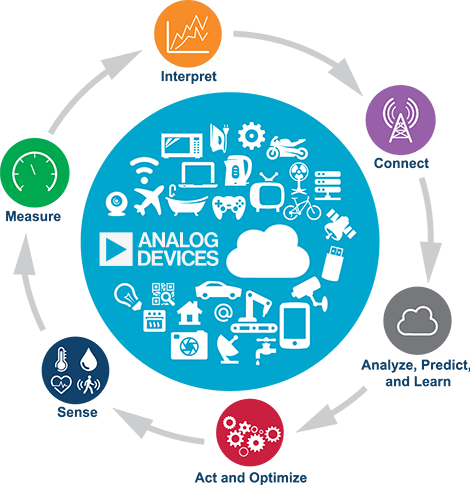
\includegraphics[width=.45\textwidth]{img/iot-cycle.png}
    \caption{Ciclo de IoT. Fonte:\cite{iot-cycle}}\label{figIoTCycle}
\end{figure}

Atualmente, a coleta de dados e uso de ferramentas de análise são o principal recursos de empresas competitivas no gerenciamento de suas atividades. Com o avanço da área de telecomunicações, as organizações têm potencial de transformar grandes volumes de dados em \textit{insights} poderosos, que orientam a tomada de decisões da equipe de gestão. Portanto, a Internet das Coisas representa uma tendência forte e disruptiva na sociedade.

Por exemplo, a Amazon\textsuperscript{\textregistered}, uma das maiores empresas de comércio eletrônico no mundo, anunciou em 2022 o lançamento do robô \textit{Sparrow}, cuja função é manipular objetos em esteiras e realizar o empacotamento
com destreza comparável à de seres humanos. Em suas fábricas, existe um crescente uso de tecnologias de ponta, como robôs autônomos e inteligência artificial, para maximizar as suas entregas em um mercado competitivo \cite{amazon-robos}.

\section{Sistemas Distribuídos}

``Um sistema distribuído é aquele no qual os componentes localizados em computadores interligados em rede se comunicam e coordenam suas ações apenas passando mensagens.'' \cite[pp. 1]{sistemas-distribuidos-coulouris2013}.
A definição apresentada pelo autor leva em conta dois importantes fatores: o primeiro é representado pela comunicação via rede de computadores, e o segundo está relacionado ao provisionamento de um serviço.
O mundo atual oferece inúmeros exemplos da importância dos sistemas distribuídos no desenvolvimento socioeconômico: a modalidade de educação à distância \cite{mec-ead}, no qual serviços web e compartilhamento
multimídia são responsáveis por possibilitar o acesso ao ensino de qualidade ao público distante fisicamente dos grandes centros de ensinos, como, por exemplo, cidades do interior ou comunidades ribeirinhas; o comércio digital, onde a arquitetura do sistema deve suportar picos de acesso em determinados períodos do ano e controle
de concorrência na compra de produtos, deve-se ao crescimento do seguimento de \textit{e-Commerce},
resultou em um faturamento superior à R\$ 180 bilhões de reais em 2023 no Brasil, de acordo com dados da Associação Brasileira de Comércio Eletrônico \cite{abcomm-ecomerce}; e redes \textit{blockchain}, pois as transações distribuídas devem ser auditáveis e transparentes, além do funcionamento descentralizado \cite{juliana-blockchain}, exemplo 
das criptomoedas, pois a tecnologia permite a transferência de recursos e o armazenamento de todas as operações.  

Portanto, o sistema distribuído tem foco no compartilhamento de recursos. Na web, a implementação de arquitetura mais comum é o modelo cliente/servidor, pois
um número grande de aplicações utiliza essa premissa, por exemplo, plataformas de redes sociais, jogos online e serviços bancários.
Ao nível do Sistema Operacional, a comunicação entre processos executados em diferentes computadores interligados em rede é essencial para o gerenciamento e acesso aos recursos distribuídos.
Nesse contexto, um cliente, que pode ser um processo ou aplicativo, realiza uma solicitação ao servidor para acessar ou manipular um recurso, como arquivos, impressoras, ou mesmo capacidade de processamento. O servidor, 
ao receber essa solicitação, desencadeia uma série de operações internas, que podem incluir desde a autenticação do cliente até a busca de dados em um banco de dados distribuído. Em seguida, o servidor 
retorna o resultado ao cliente em espera, completando o ciclo de comunicação do tipo requisição/resposta \cite[pp. 16]{sistemas-distribuidos-coulouris2013}.

\section{Protocolo HTTP}

O HTPP (do inglês \textit{HyperText Transfer Protocol})

\section{AOSP}

AOSP é coisa e tal

\section{Desenvolvimento Android}

Android é coisa e tal 

\section{ESP32 e NodeMCU}